\documentclass[a4paper, 11pt, oneside, openany, ngerman, onecolumn]{scrbook}

\usepackage[ngerman]{babel}
% Positionierung von Bildern
\usepackage{float}
% Bib
\usepackage{natbib}
% Tabelle formatieren
\usepackage{tabularx}
% Bilder einfügen
\usepackage{graphicx}
% URLs, Zeilenumbruch auch bei Bindestrichen
\PassOptionsToPackage{hyphens}{url}\usepackage[pdfencoding=unicode]{hyperref}
% Rechtschreibprüfung
\usepackage{spelling} 
% Quellcode einbinden
\usepackage{listings}
% Farben
\usepackage[table]{xcolor}
% TODO-Marker
\usepackage{todonotes}
% Subfigures
\usepackage{subcaption}
% Math
\usepackage{mathtools}
% Für Header
\usepackage{fancyhdr}
\graphicspath{ {./images/} }
\pagestyle{fancy}
\fancypagestyle{plain}{}
% Header
\rhead{Tomas Daetz}
\lhead{\today}
\chead{tj18b}
\renewcommand{\headrulewidth}{0pt}
% Foot
\renewcommand{\footrulewidth}{0pt}

\renewcommand{\clearpage}{}
\vspace{\baselineskip}

\definecolor{stringcolor}{RGB}{0,150,20}
\definecolor{keywordcolor}{RGB}{0,90,230}
\definecolor{commentcolor}{RGB}{192,32,32}

\setlength{\parindent}{0em}
\setlength{\parskip}{1em}
\setlength{\extrarowheight}{5pt}

\begin{document}
\sloppy

\frontmatter
\begin{titlepage}
	\begin{center}
		{\Huge\textbf{Qualitätssicherungskonzept}\vspace{2em}}

		{\Large\textbf{Synchronisation und Auswertung von Roboterfußballvideos}\vspace{1em}}

		{\textsf{tj18b}\vspace{2em}}

		\begin{table}[b]
			\begin{tabularx}{\textwidth}{lXr}
				\textbf{Mitglieder}&&\textbf{Betreuer}\\
				Dan Häßler&&Hans-Gert Gräbe\\
				Robert Wagner&&Tobias Wieprich\\
				Sirk Petzold&&Tobias Jagla\\
				Alex Eichhorn&&André Köhler\\
				Erik Diener&&\\
				Jonas Wrubel&&\\
				Tomas Daetz Chacon&&\\
			\end{tabularx}
		\end{table}
	\end{center}
\end{titlepage}

\tableofcontents


\mainmatter
\newpage
\chapter{Installation}
\section{Dependencies}
OpenCV 3.4.1 oder aktueller wird zum Ausführen benötigt.

\section{Systeme}
Das Programm läuft unter folgenden Systemen:
\begin{itemize}
\item Windows
\item Ubuntu 18.04
\item MacOS
\end{itemize}  

\section{Einrichtung}
\subsection{Für Windows und MacOS}
\begin{enumerate}
	\item Kommandozeile im Ordner der Sources öffnen.
	\item Befehl ausführen: \\ mvn package
\end{enumerate}
\subsection{Für Linux:}
Leider müssen Linux Nutzer OpenCV selbst herunterladen und bauen. Dazu muss man folgende Schritte folgen: \\
\begin{enumerate}
	\item OpenCV Sources 3.4.1 oder aktueller von \href{https://opencv.org/releases.html}{hier}  herunterladen.
	\item Inhalte in einem Ordner entpacken.
	\item Kommandozeile öffnen und folgenden Befehl ausführen:\\ cmake -D BUILD\_SHARED\_LIBS=false <Pfad zum Ordner von Schritt 2>
	\item Letzten Befehl ausführen:\\ make -j4
	\item Anschließend den Schritten von dem Abschnitt für Windows und MacOS folgen.
\end{enumerate}

\section{Ausführen}
\subsection{Windows}
java -javaagent:WinFixAgent.jar -jar SyncGod-3.0.jar
\subsection{Andere Systeme}
java -jar SyncGod-3.0.jar


\input{Leistungsvermögen.tex}
\chapter{Nutzung}
In diesem Kapitel werden die Funktionen und Optionen des Programms ausführlich erklärt. 
Zuerst folgt eine Beschreibung der Menüleiste und der Möglichkeiten, Dateien in das Programm zu laden. Anschließend folgt eine Beschreibung der einzelnen Programmbereiche.
\\
\section*{Menüleiste}

\section{Open Project}
Über diese Schaltfläche kann ein bereits begonnenes Projekt geladen werden. Es werden lediglich MLT Dateien geöffnet.\\
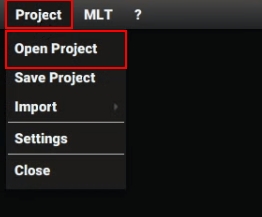
\includegraphics[width=7 cm]{menu_open_project.png}

\section{Save Project}
Diese Schaltfläche ermöglicht das Speichern eines begonnenen Projektes, mit der Möglichkeit eine spätere Bearbeitung vorzunehmen. Es wird als MLT Datei gespeichert.\\
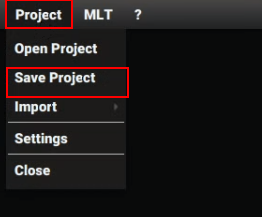
\includegraphics[width=7 cm]{menu_save_project.png}
 
\section{Import}
Das Programm bietet verschiedene Ladeoptionen für Dateien an. \\
\subsection{Laden über die Menüleiste:}
Durch die Auswahl der Project-Schaltfläche oben links in der Menüleiste und der anschließenden Auswahl der Schaltfläche Import hast du die Möglichkeit, nach der Wahl zwischen Video, Picture und GC Log über ein weiteres Fenster die gewünschten Dateien auszuwählen. Hierbei ist es möglich, mehrere Videos gleichzeitig zu markieren. 
\\
\vspace{5mm}
\\
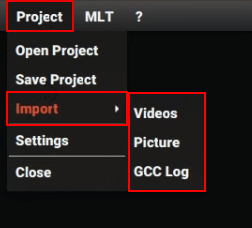
\includegraphics[width=7 cm]{menu_imports.png}\\

\subsection{Laden über die Drag and Drop Funktion:}
Die Videos und die Log-Datei können auch per Drag-and-Drop direkt in den entsprechenden Bereich des Programmes gezogen werden. Dabei ist der rechte Bereich für die Log-Datei, der linke Bereich für die Videos vorgesehen.
\\
\vspace{5mm}
\\
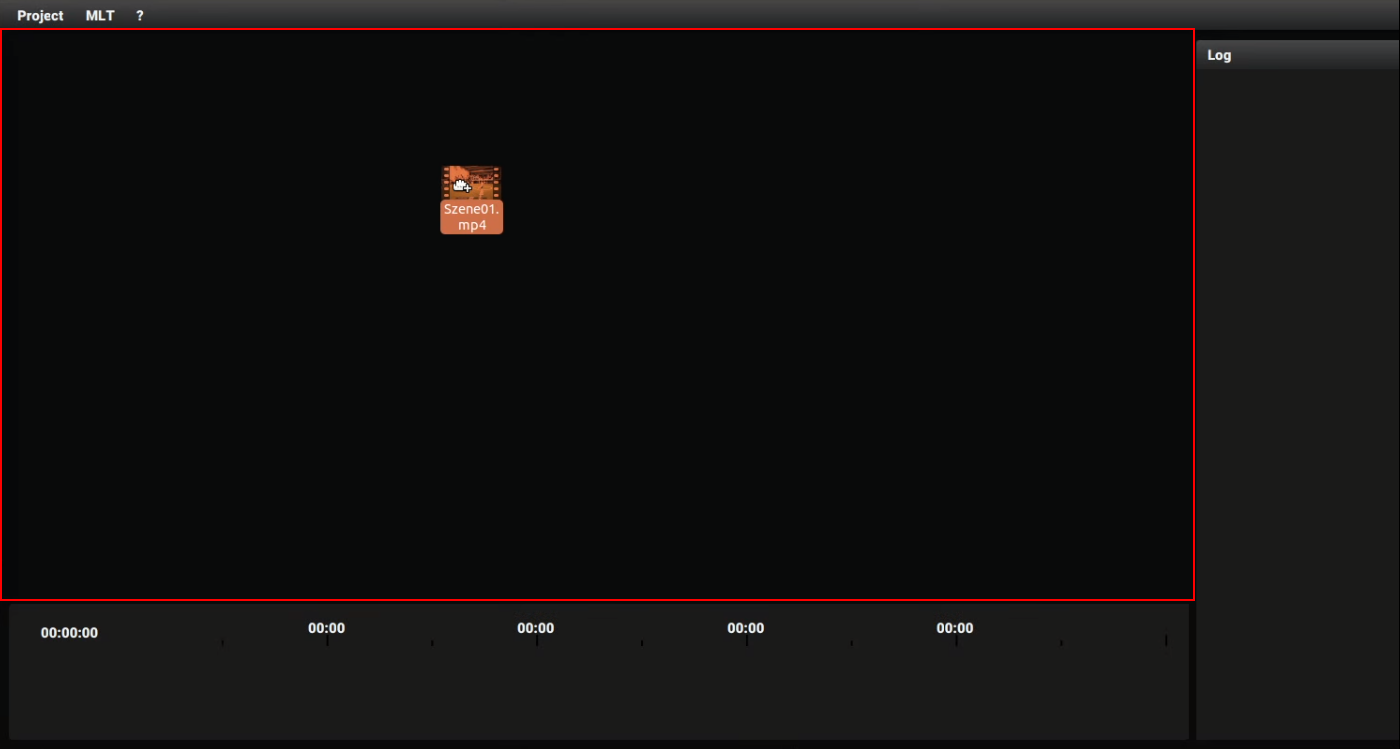
\includegraphics[width=7 cm,height=6 cm]{dragndropvideo.png}
\hspace{20mm}
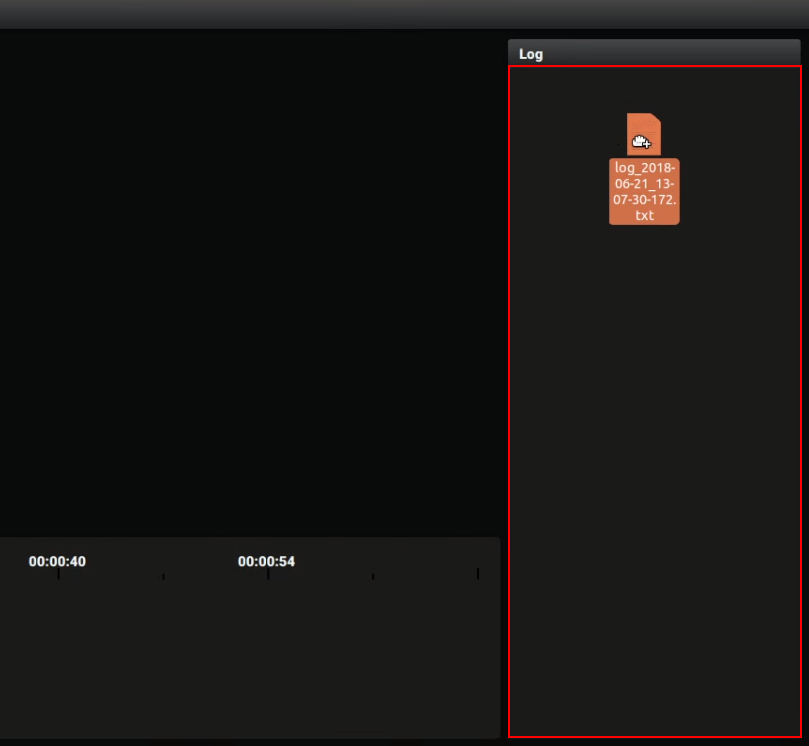
\includegraphics[width=4 cm,height=6 cm]{dragndroplog.png}\\

\section{Settings}
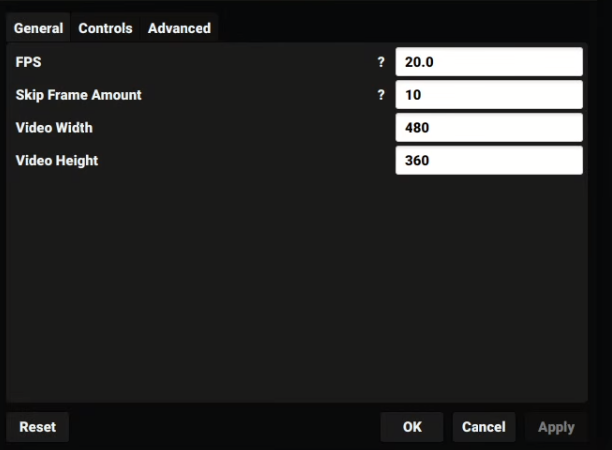
\includegraphics[width=10 cm,height=6 cm]{settings_menu1.png}\\
\\ 
In dem General-Tab der Settings kannst du allgemeine Einstellungen bezüglich der Videos treffen. \\
\textbf{FPS : } Die Frames pro Sekunde, welche in vielen Bereichen des Programmes verwendet wird. Die geladenen Videos sollten diese FPS Zahl haben.\\
\textbf{Skip Frame Amount : }	Stellt die Anzahl der zu überspringenden Frames ein, wenn \hspace{5mm} \ll \hspace{5mm}  oder  \hspace{5mm}   \gg \hspace{5mm}gedrückt wird. \\
\textbf{Video Width/Height : } Die Breite und Höhe der einzelnen Videos kann hier angepasst werden.
\\
\vspace{5mm}
\\
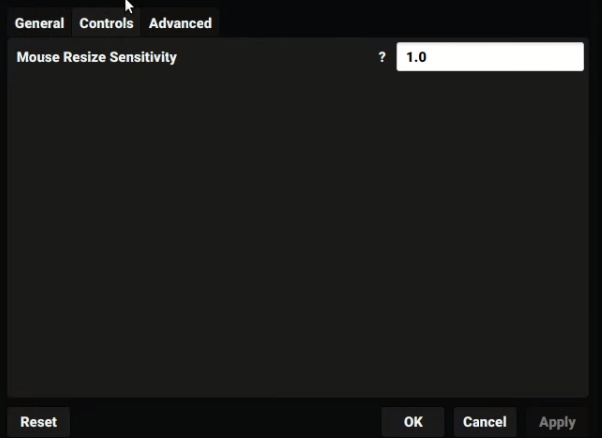
\includegraphics[width=10 cm,height=6 cm]{settings_menu2.png}\\
\\
Der Controls-Tab der Settings ermöglicht Einstellungen zu verschiedenen Tastenkürzeln für einzelne Funktionen sowie Sensitivitätseinstellungen der Maus. \\
\textbf{Mouse Resize Sensitivity : } Setzt die Mausempfindlichkeit für die Markierungen innerhalb der Track-Box.\\

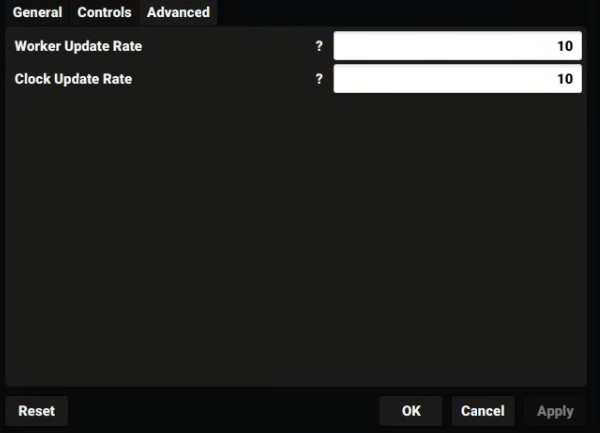
\includegraphics[width=10 cm,height=6 cm]{settings_menu3.png}\\
\\
Unter dem Advanced-Tab der Settings können Feineinstellungen bezüglich der Verarbeitung getroffen werden. \\
\textbf{Worker Update Rate : } Die Videos überprüfen in der Frequenz der hier in Millisekunden eingestellten Zeit, ob das nächste Bild angezeigt werden muss oder nicht. Eine höhere Zahl verbessert die Performance, führt jedoch zu Ungenauigkeiten. Der empfohlene Wert liegt zwischen 10ms und 20ms.\\
\textbf{Clock Update Rate : } Die Synchronisierung der Videos erfolgt anhand der hier in Millisekunden eingestellten Frequenz. Auch hier ist durch eine Erhöhung des Wertes eine Performance-Verbesserung erreichbar, jedoch resultieren daraus Ungenauigkeiten. Die Empfehlung liegt bei 10ms - 30 ms.\\

\section{Help}
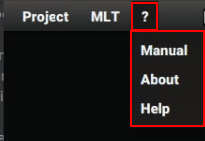
\includegraphics[width=7 cm]{menu_help.png}\\
\subsection{Manual}
Im Manual steht eine ausführliche Beschreibung sämtlicher Funktionen des Programms.\\
\subsection{About}
Hier befindet sich eine allgemeine Übersicht über Version, BuildTool, Website, als auch eine Liste der beteiligten Developer. \\
\subsection{Help}
Eine Einführung und Schnellhilfe mit nützlichen Kurztipps zu einzelnen Funktionen. 
\section*{Programmaufbau}
\section{Log-Anzeige}
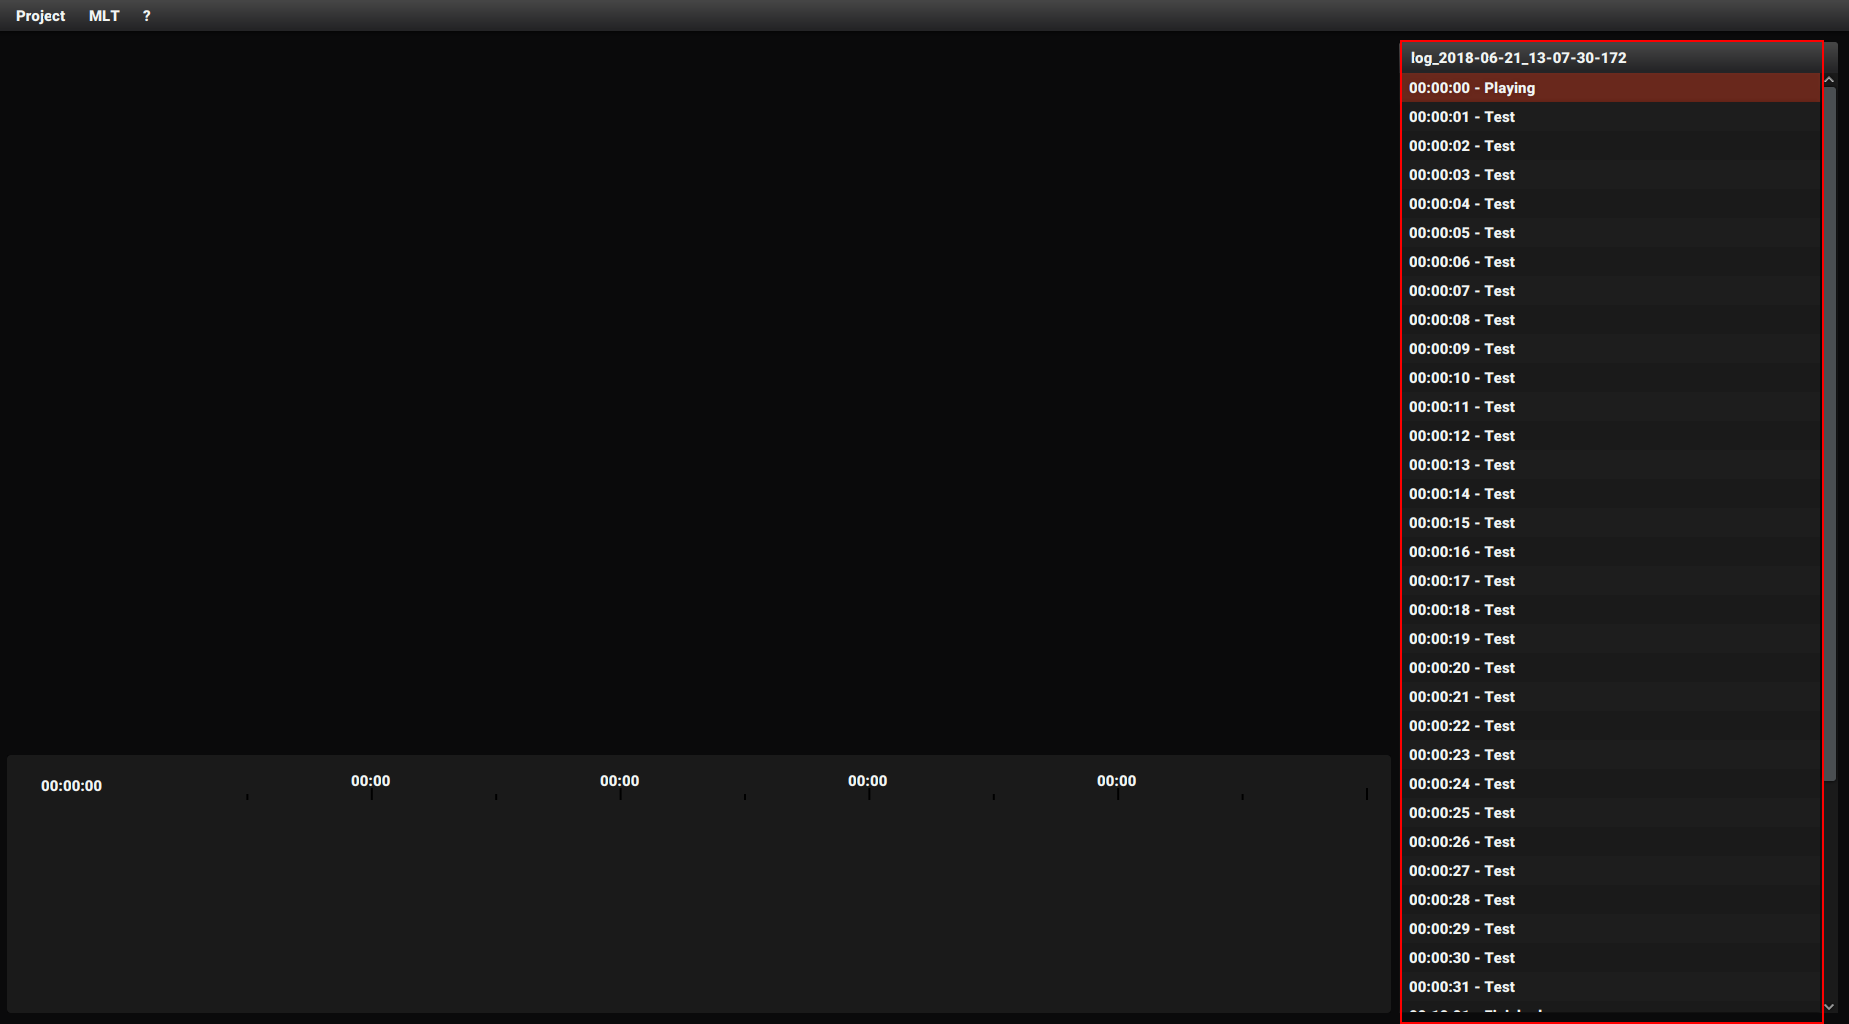
\includegraphics[width=10 cm,height=6 cm]{log.png}\\
\\
Die Log-Anzeige stellt das GC-Log graphisch dar.\\
Bei der Wiedergabe der Videos ist die Markierung in der Log-Anzeige mit den Videos synchronisiert. \\
Durch die Auswahl eines Events im Log springen die Videos zu diesem Event und werden pausiert. \\
 
\section{Video-Anzeige}
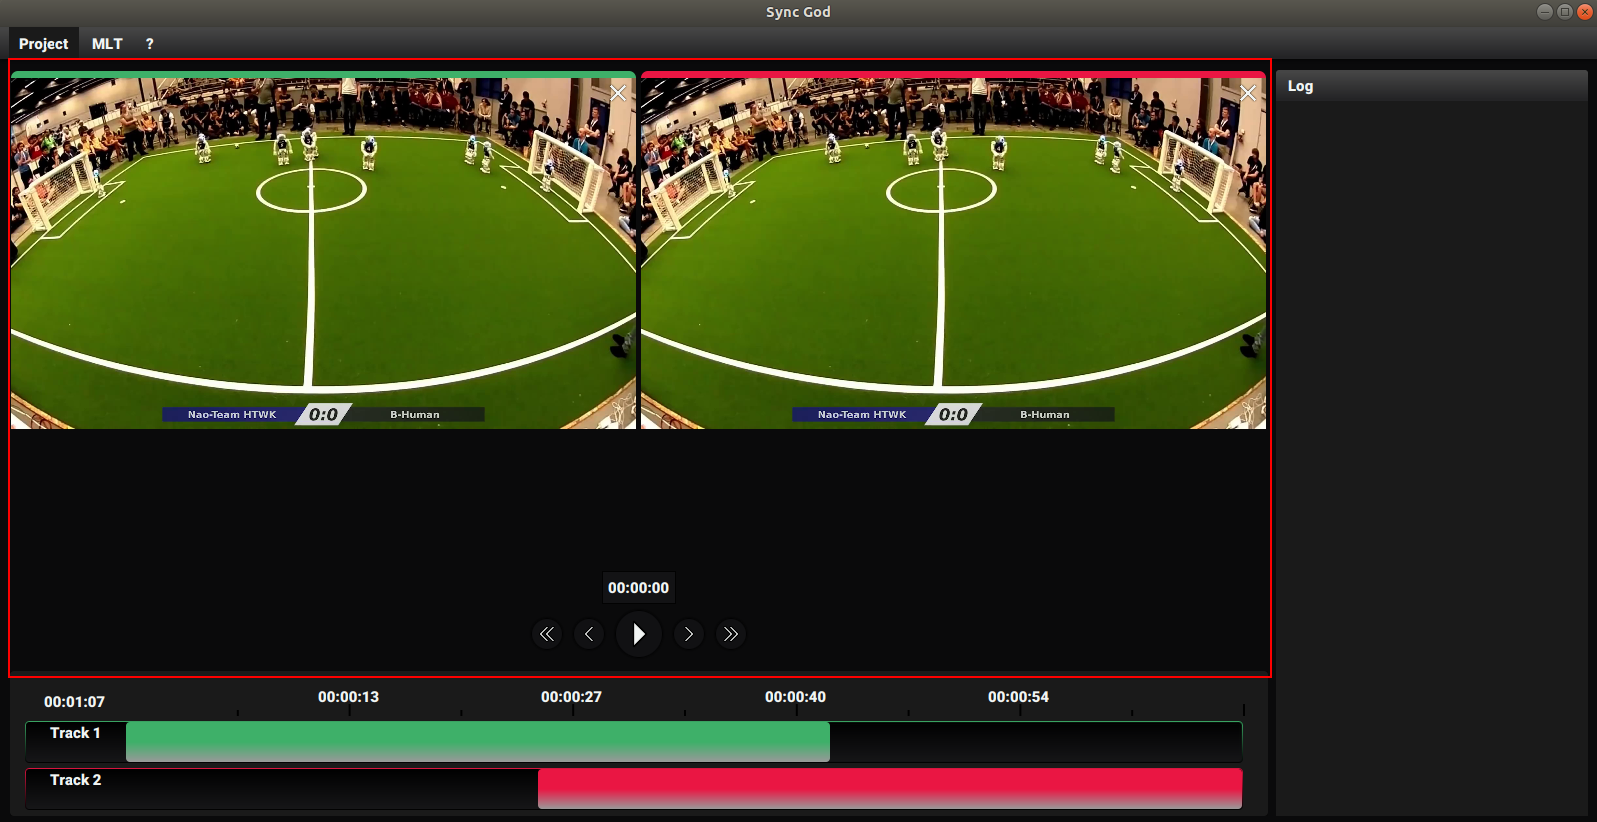
\includegraphics[width=10 cm,height=6 cm]{video_screen.png}
\vspace{5mm}
\\
Die Video Anzeige stellt die ausgewählten Videos nebeneinander und synchronisiert dar.
Bei dem Laden der Videos muss für jedes eine Eingabe zum Offset getätigt werden.

\section{Track-Anzeige}
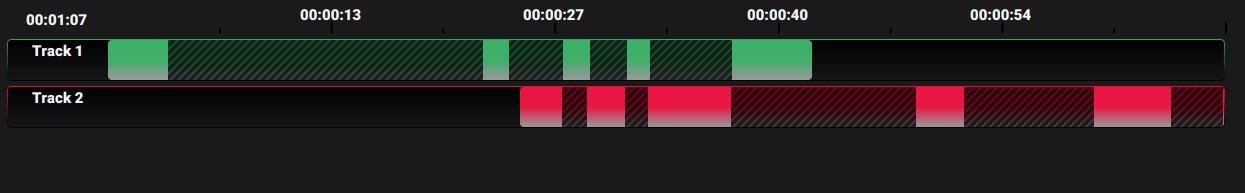
\includegraphics[width=14 cm,height=2 cm]{track_screen.png}
\vspace{5mm}
\\
Die Track-Anzeige stellt die Videos in Beziehung zueinander dar. Verschiebungen durch Offsets werden beachtet. Dabei wird ein Track erstellt, wenn ein Video hinzugefügt wurde.\\
Die Farbe des jeweiligen Tracks stimmt mit der Farbe am oberen Rand des dazugehörigen Videos überein. \\
Abschnitte der Tracks können mit der Maus per gehaltener linker Maustaste und ziehen über den gewünschten Bereich markiert werden. Eine Markierung bedeutet, dass dieser Bereich des Videos für die spätere Weiterbearbeitung verwendet wird.    \\
Ein doppelter Klick der rechten Maustaste auf einen der Bereiche entfernt diese Auswahl wieder. \\
Wenn eine Markierung in einem Bereich gesetzt wird, welche Bereiche anderer Markierungen in anderen Tracks überdecken, so wird die Überlappung bei den alten Tracks entfernt.   
\section{Export}
Die MLT Datei kann über die MLT Schaltfläche in der Menüleiste generiert werden.\\

\includegraphics[width= 7 cm]{menu_mlt.png}

\chapter{Wartung}

\section{Mögliche Probleme während der Nutzung}
Manchmal werden beim Laden eines MLT nicht die Markierungen von den Trackboxen gezeigt. Dies lässt sich jedoch mit einem Click auf die Trackbox lösen. 
\section{Weiterentwicklung/Schnittstellen}

\section{Beachtenswertes}

\end{document}